\section{Workshops}

\subsection{Workshop Setup}

\input{chapter4_methods/sections/figures/Mapping Setup}

The section above details our motivations to employ participatory mapping as a tool to explain and question geospatial civic AI. To conduct participatory mapping sessions, I used an existing tool named MapSpot  \cite{Mapspot}, a part of the Atlanta Map Room Project \cite{maproom}. This project is an expansion of the St.Louis Map Room \cite{stmaproom}, that brings together local community members to explore and represent the relationships between civic data and lived experiences. This grassroots mapping effort aims to problematize the “objective” and “stable” nature of big data and grounds data and its limits in contextual experiences of space. 

In our mapping sessions, participants gathered around a mapping set-up that included a table covered with drawing paper and a short-throw projector turned 90 degrees to project a digital map on the table. The projection acted as a guide for participants to map spatial components related to AI systems. On this paper, participants mapped their place-based experiences of safety and how they may relate to spatial algorithmic predictions. The projected digital, as part of the Mapspot tool \cite{Mapspot}, also allowed us to overlay data layers onto the mappings of participants including demographic data such as census data or historical data such as red-lining maps (see \cref{fig:mapspot_webpage}). Such superimposition of grounded local data and institutional data allowed the group to understand if and how space, and the people who live there, would experience predictive technologies differently. 

\input{chapter4_methods/sections/figures/Mapspot_webpage}

\subsection{Pilots}

% \begin{wrapfigure}{r}{0.5\textwidth}
\begin{figure}[ht]
% \hfill
    \begin{subfigure}[b]{0.5\linewidth}
         \centering
         \includegraphics[width=0.99\linewidth]{chapter4_methods/sections/images/DM_Demo.jpeg}
         % \caption{John Snow's map that traces the spread of Cholera deaths during London's 1854 Cholera epidemic}
         \label{dmdemo:subfig1}
    \end{subfigure}
    \begin{subfigure}[b]{0.5\linewidth}
         \centering
         \includegraphics[width=0.99\linewidth]{chapter4_methods/sections/images/GVU_Demo.jpg}
         % \caption{John Snow's map that traces the spread of Cholera deaths during London's 1854 Cholera epidemic}
         \label{dmdemo:subfig2}
    \end{subfigure}

    
% \hfill
    % \begin{subfigure}[b]{0.49\linewidth}
    %      \centering
    %      \includegraphics[width=0.95\linewidth]{images/Snow-cholera-map_resized15.jpg}
    %      % \caption{}
    %      \label{subfig2}
    % \end{subfigure}
% \hfill
% \centering
% \includegraphics[width=0.45\textwidth]{images/REDUCEDD_Snow-cholera-map}
\caption{
    Pilot study sessions conducted as part of Digital Media Demo Day (left) and GVU Research Showcase (right) in April 2023
}
\label{fig:dmdemo}
\end{figure}
% \end{wrapfigure}
% \ref{fig:choleramap}  

I conducted two pilot mapping sessions in April 2023 that focused on the design and impacts of place-based predictive policing tools. These sessions were conducted as part of the Digital Media Demo Day \cite{DMDemoday} and the GVU Research Showcase \cite{GVUDemoday} on the main campus of the Georgia Institute of Technology in Atlanta, GA. These demos were done in an exhibit setting and the mapping sessions typically lasted between five and twenty minutes with participant groups ranging between one and five participants. In total, approximately twenty people actively participated. 

Participants included Georgia Tech alumni and other industry, government, academic, and civil service individuals who were interested in learning more about the projects and research happening at Georgia Tech. Demographic details of the participants were not collected due to the format of the interactions. However, by virtue of the places and networks where these events are advertised as well as the voluntary sampling of people, it can be estimated that the audience was more technically savvy or interested in learning more about how humans and computers interact. 

The goal of the pilot studies was to understand if a participatory mapping activity shows potential to investigate the research question this dissertation asks: \emph{How can the Explainable AI (XAI) community support public understanding of the spatial workings and effects of civic predictive systems? }. To do so, participants engaged in a speculative exercise where they imagine and discuss how a predictive system may categorize the places they know and live on on the map and why.  

Through this exercise, I found that participants were able to ask critical questions about AI systems and their spatial effects. Some examples include: inquiring about the impacts of over-reporting and under-reporting of crime and on AI predictions; questioning the ends towards which these predictions are used (increasing police presence or systemic change); or discussing predictions for white collar crime data vs blue collar crime data. 

Participants also reflected on participatory mapping and speculative personation as a methodology in supporting such critical thinking. A participant said: 

\begin{quote}
    I think the interactive piece helps ground this in their own experience to think about ok.. where do I live.. where my actual life took place in this area. So I can actually think about streetlights and bus stops and things like that.
\end{quote}

It was considered an ``\textit{excellent way of }\textit{getting the conversation and pulling it out of people}". Another aspect participants discussed was the embodied nature of the personation experience and expressed discomfort in making algorithmic predictions. For instance, a participant said: 

\begin{quote}
    I think for me forcing me to draw areas that I think would be flagged was like really fascinating.. I did not want to do that cuz I was like.. there was some uncomfortableness in doing that. 
\end{quote}

Speculative personation using maps allowed participants to reflect on the moral responsibility of making high impact predictions, a responsibility that can never be felt by AI systems as they cannot feel \cite{veliz2021moral}. 

These early pilot studies showed promise in the use of participatory mapping and speculative personation for collectively understanding AI systems and the broad socio-technical assemblages that surround them. Following these demo pilots, I conducted a workshop with Georgia Tech students as a dry run leading up to five primary workshops that inform the rest of my dissertation. I report on these workshops below. 

\subsection{Workshops}

Five workshops were conducted in person in Atlanta, Georgia located in the Southeast United States. The groups who participated in the workshops were invited through one of the following ways: (1) they were recruited through open calls for participation which were shared with numerous non-profits and civic organizations via email, (2) they had existing relationships with the authors and authors reached out to ask if they would be interested in participating, and (3) they were familiar with the ongoing work of the authors and reached out to participate. The workshops were conducted as one-time 90-minute workshops in either the offices of participating organizations or the university campus of the authors. I led the moderation of every workshop with organizational and documentation support from colleagues. The workshops were audio and video recorded. The study was approved by Georgia Tech's IRB.

Before each workshop, a short survey was shared with the participants. The survey served two primary purposes: (1) it confirmed participation through an informal registration process, and (2) it provided workshop moderators with background information that was helpful for unique workshops (see Appendix B). The survey asked participants about the Atlanta neighborhoods they were familiar with so I can focus our conversation on those areas, their goals for participation, their familiarity with AI tools, and any existing questions, opinions or concerns they had about AI systems. This information helped me, and my fellow moderators, in understanding the explanation contexts we would be moderating. 

The workshops started with participants engaging in what I call `speculative personation'. They were asked to make spatial predictions as an AI system would. They identified places on the map that they were familiar with and believed a predictive tool may identify as crime hotspots. They were then asked to reflect on their predictions by considering their reasoning and effects. The workshops followed a loose protocol that guided such reflection. Participants contemplated an AI system's prediction goal, data type, data source and amount, spatial aggregation of data, and prediction effects in relation to their own speculations. In doing so, moderators prompted participants to consider the socio-political qualities of places they identified in relation to these technical aspects of the AI system. A focus on specific locations revealed spatial, social, political, and historical characteristics relevant to the technical workings of the predictive tool. The protocol was documented as a toolkit and shared as a take-away artifact with the workshop participants to support their questioning of AI systems beyond the workshops (see Appendix C). In Workshop 3, I introduced another page to the artifact that provided information on other AI powered public safety tools in the US, if and when were they used in the city of Atlanta, and a one-sentence description of media articles that document their real-life impacts. The need for this information was felt in the earlier workshops as participants discussed public safety AI more broadly. It is essential to note that this structure of the toolkit was not rigid and merely acted as a guide to the conversation while allowing the group to deviate into explaining and questioning components of AI systems that were most relevant.

 I, with the support of my colleagues, conducted workshops with a Police Reform Group (Workshop 1 or W1), City Planners (W2), Neighborhood and Civic Representatives (W3), a Community Development Organization that funds technology innovation projects (W4), and Educators part of an education non-profit (W5).  In chronological order, I describe these workshops below. 
 
% TODO (@nirbhay): Insert 4x4 table here 
\begin{table}[h!]
\setlength\extrarowheight{1mm}
\begin{tabularx}{1.0\textwidth}{lXll}
\toprule
Workshop & Group & Participant Count & Timeline \\
\midrule
Pilots & Georgia Tech Demo Days & $\approx$ 20 & Apr 2023 \\
W1 & Police Reform Group & 12 & Oct 2023 \\
W2 & City Planners & 7 & Nov 2023 \\
W3 & Neighborhood and Civic Representatives & 7 & Nov 2023 \\
W4 & Community Development Organization & 11 & Jan 2024 \\
W5 & Educators & 8 & Jan 2024 \\
\bottomrule
\end{tabularx}
\caption{Participatory Mapping Workshops conducted as part of this dissertation}
\label{tab:edit-this-tag}
\centering
\end{table}

\subsubsection{Workshop 1: Police Reform Group} 

\input{chapter4_methods/sections/figures/W1}

% \begin{wrapfigure}{r}{0.5\textwidth}
\begin{figure}[ht]
% \hfill
    \begin{subfigure}[b]{0.99\linewidth}
         \centering
         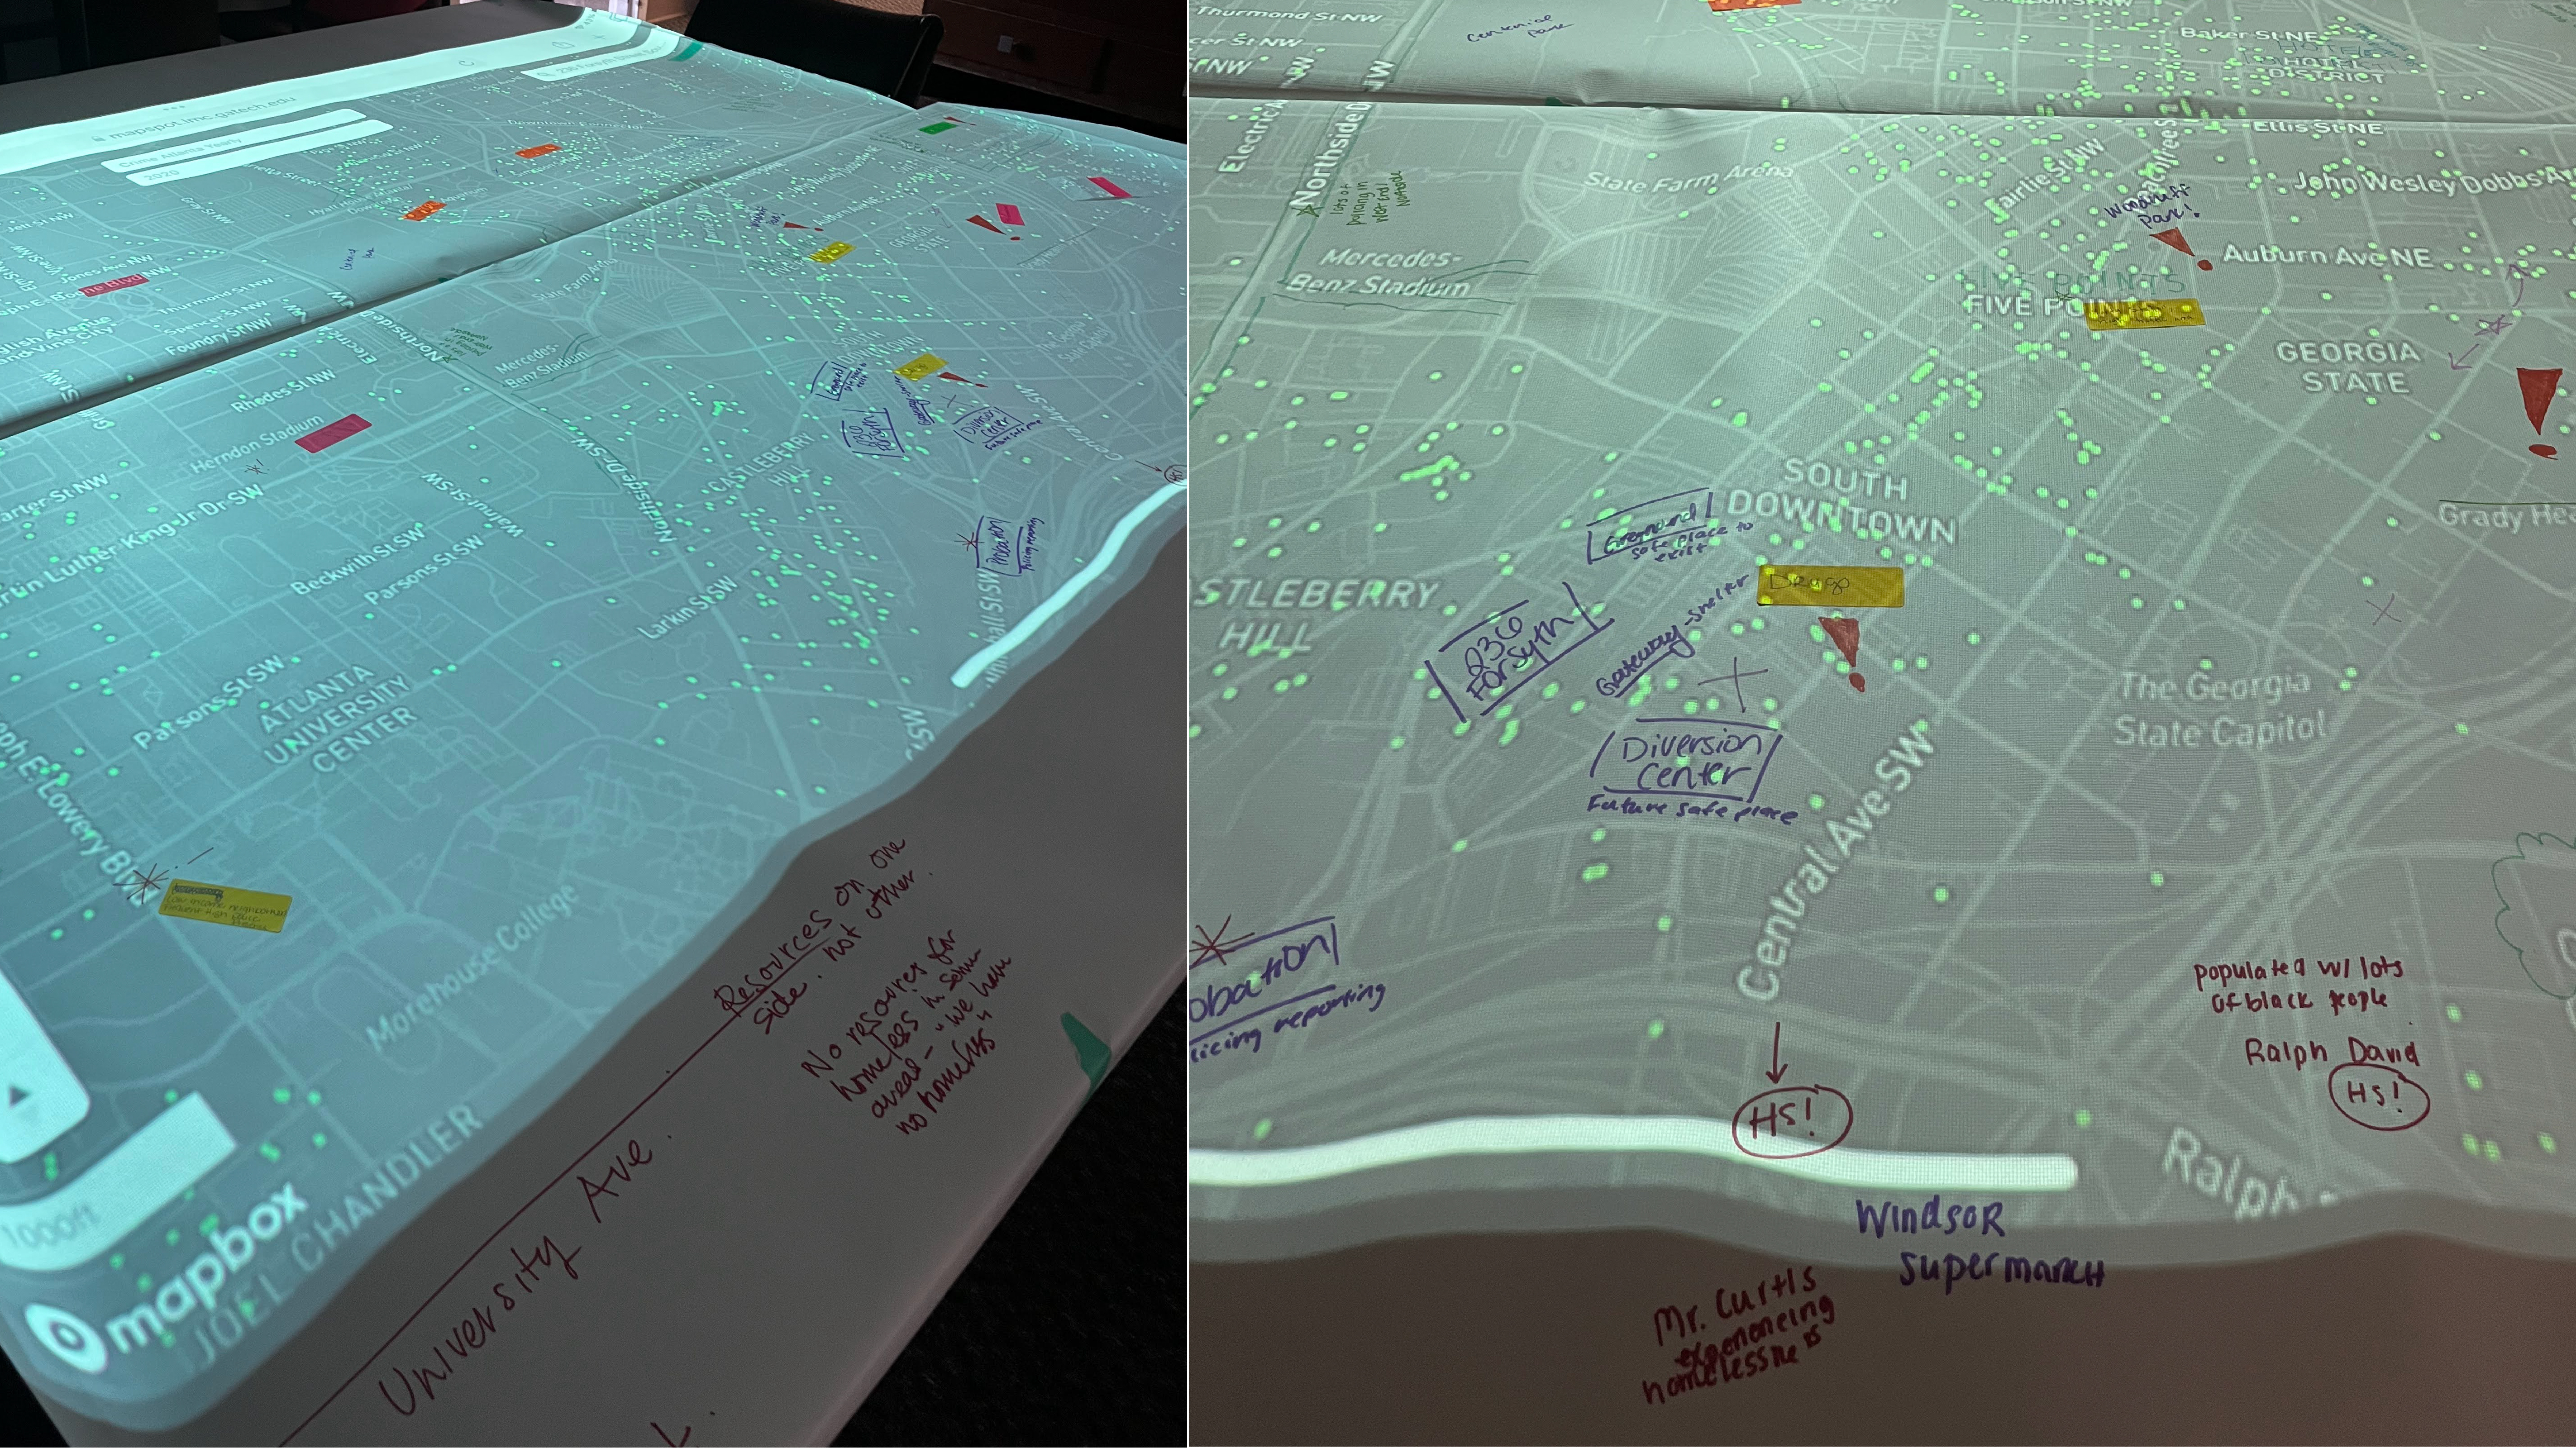
\includegraphics[width=0.99\linewidth]{chapter4_methods/sections/images/Map_closeups.jpg}
         % \caption{John Snow's map that traces the spread of Cholera deaths during London's 1854 Cholera epidemic}
         \label{subfig1}
    \end{subfigure}
% \hfill
    % \begin{subfigure}[b]{0.49\linewidth}
    %      \centering
    %      \includegraphics[width=0.95\linewidth]{images/Snow-cholera-map_resized15.jpg}
    %      % \caption{}
    %      \label{subfig2}
    % \end{subfigure}
% \hfill
% \centering
% \includegraphics[width=0.45\textwidth]{images/REDUCEDD_Snow-cholera-map}
\caption{
    Participatory Maps Close-ups
}
\label{fig:inundation}
\end{figure}
% \end{wrapfigure}
% \ref{fig:choleramap}

W1 invited twelve members of a police reform group that offers supportive services to those experiencing extreme poverty, problematic substance use, or mental health concerns, with the goal of reducing their arrest and incarceration rates. This workshop was conducted in October 2023 in the offices of the partnering organization in Atlanta. Before the workshop, I conducted a 30-minute call with the director of the group to understand their goals, motivations, and expectations of the workshop. 

In their survey, participants reported that they want to learn about the new and advanced methods in policing, what is AI and how AI will be used to promote public safety, how to use these tools responsibly, and how it can help them better serve their communities. A few of them explicitly stated that they had concerns about the use of AI in policing, especially because of the effect of racism on policing, and saw this workshop as a place to discuss those concerns. Participants described themselves as having 'none' to 'very little' knowledge of AI. Two mentioned their use of ChatGPT and another talked about their knowledge of policing technologies like surveillance cameras. 

\subsubsection{Workshop 2: Urban planners} 

\input{chapter4_methods/sections/figures/W2}

W2 invited seven members of a regional civic planning agency in Atlanta.  It supports the leaders of Atlanta in using data-driven methods to plan, invest, and addresses critical issues for the betterment of city's collective future. The workshop took place in the first week of November 2023 in the offices of the organization based in Atlanta. 

Participants were interested in learning about how AI can be used for the betterment of the city and promote equity. They mentioned their roles as urban planners and designers and sought knowledge of civic AI tools to skillfully engage with these tools in their professional work.  Five participants described themselves as being familiar with AI through podcasts, readings, use of ChatGPT, their own work, or the work of those around them. The group seemed excited about the opportunities offered by AI but wanted to learn about how to design, deploy, and use sch tools in an equitable manner.  

\subsubsection{Workshop 3: Open Call} 

\input{chapter4_methods/sections/figures/W3}

Unlike the rest of the workshops, W3 was an open call workshop publicized via a webpage, email, and flyers with neighborhood association leaders, board members, and other neighborhood and civic groups. Folks were encouraged to share and publicize the workshop details to anyone in their network who they deem would be interested. The workshop received seventeen registrations of which seven people participated in the workshop. The workshop was organized on the Georgia Tech campus in mid November. 

This workshop saw a wider range of people. The participants included researchers and practitioners from both academia and civic organizations for neighborhood improvement. One participant worked in violence prevention in Atlanta and another was leading a neighborhood public-private partnership aimed at making spaces better for citizens.  In the survey, some described themselves as ``Pretty familiar with usage" of AI tools and others as ``Not very familiar" with AI. Some had friends who worked in AI and others had used tools with predictive features. Participants were interested in how AI could be used for civic purposes in responsible ways. Two participants were aware of the biases that can creep into AI systems and considered the workshop a space to learn and talk more about it. This workshop was met with a technical error where our short-throw projection on the table stopped working and I, along with my co-moderator, improvised to a wall displayed map. 

\subsubsection{Workshop 4: Community development organization} 

\input{chapter4_methods/sections/figures/W4}

W4 brought in eleven members of an organization that leads, manages, and funds local, community-centered projects across Georgia. This workshop was organized as part of an annual retreat for the organization members where members gathered to discuss strategy for the rest of the year. The organization director met with me before the workshop and considered the workshop timely and useful for members to understand how AI systems may affect the city. Such an understanding, the director hoped, would support their work in civic development for the smart city. The workshop was organized in their offices in early January 2024. 

Most people were participating as the workshop was included as a part of their team retreat. They were interested in incorporating the learnings from the workshop into their work. Participants mentioned different predictive tools they were familiar with. Three participants mentioned variations of ChatGPT, Claude or Bard while some talked about Google maps and Google translate. Overall, the group presented themselves as being familiar with AI through various articles they read, tools they have used, collaborations with AI researchers, or their own work in smart cities. One participant described their interest in learning how to make these tools transparent to the public. Another talked about the privacy and safety of these tools rural communities. 


\subsubsection{Workshop 5: Non-profit of educators} 
\input{chapter4_methods/sections/figures/W5}

W5 invited a group of eight teachers who came together as a non-profit aimed at forming meaningful relationships and collaborations between educators. The non-profit leaders offer experiences to support teachers in their work and, with this workshop, hoped to come together to learn more about AI and its effects on cities. The workshop was organized on the Georgia Tech campus in late January 2024. 

Participants wanted to learn how to responsibly incorporate AI in their teachings, especially with the rise in generative AI and its effect on education. Two teachers taught geography, another taught social science. One participant said they had ``not given AI a great deal of thought", while another participated in a school committee to discuss AI use in high school education. 

 Three of the five workshop partners posted about this work on their social media channels reflecting on their experience and demonstrating the impact the workshop had such as: 

\begin{quote}
    ``As we look to the future of these technologies, we have the potential to enhance community well-being and resource distribution, but only if we fully understand their potential and limitations.'' (W4)
\end{quote}

\begin{quote}
   ``Our engagement [through the workshop] not only broadened our understanding of the power of maps and the ethical implications of AI but also served as a reminder of our role as educators in shaping future perspectives.'' (W5)
\end{quote}



These workshops together inform the rest of the work discussed in this dissertation. I analyse these workshops through two primary methods (1) situational analysis and (2) thematic analysis and memo-ing which I discuss in Chapter 4 and Chapter 5 respectively.